\documentclass[tikz,border=10pt]{standalone}
% Scale: s = 0.012882 cm/px, centre (cx,cy) = (367,364) px, y flipped
\begin{document}
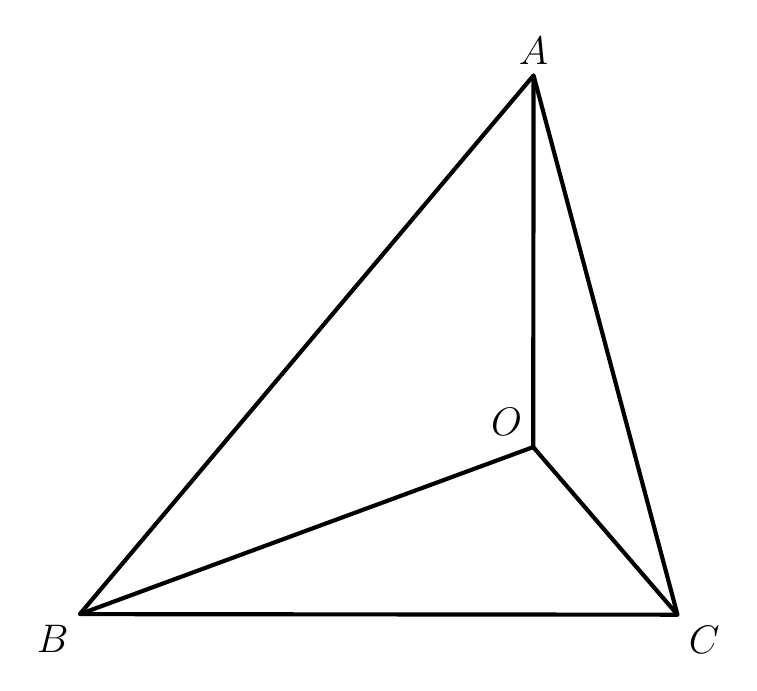
\begin{tikzpicture}[line width=1.5pt, line join=round]
  % Named vertices (converted from pixels)
  \coordinate (A) at (1.9722422299241744,3.429997869660911);     % A (519.97,97.84)
  \coordinate (B) at (-3.7900013247935505,-3.4113943757568075);   % B (72.56,628.78)
  \coordinate (C) at (3.8000013247935502,-3.4186056242431926);    % C (662.12,629.28)
  \coordinate (O) at (1.9677577700758255,-1.2899978696609111);    % O (520.17,464.3)

  % Triangle ABC, no fill
  \draw (A) -- (B) -- (C) -- cycle;

  % Vertical altitude from A to O
  \draw (A) -- (O);

  % Cevians from B and C end exactly at O
  \draw (B) -- (O);
  \draw (C) -- (O);

  % Labels
  \node[above, font=\fontsize{15}{18}\selectfont] at (A) {$A$};
  \node[below left, font=\fontsize{15}{18}\selectfont] at (B) {$B$};
  \node[below right, font=\fontsize{15}{18}\selectfont] at (C) {$C$};
  % O label upper-left of the point, touching BO
  \node[above left, font=\fontsize{15}{18}\selectfont] at (O) {$O$};
\end{tikzpicture}
\end{document}